\documentclass[a4paper,12pt]{article}

\usepackage[margin=2.5cm]{geometry}  % change page margins

%%% Работа с русским языком
\usepackage{cmap}					% поиск в PDF
\usepackage{mathtext} 				% русские буквы в формулах
\usepackage[T2A]{fontenc}			% кодировка
\usepackage[utf8]{inputenc}			% кодировка исходного текста
\usepackage[english,russian]{babel}	% локализация и переносы

%%% Дополнительная работа с математикой
\usepackage{amsfonts,amssymb,amsthm,mathtools} % AMS
\usepackage{amsmath}
\usepackage{icomma} % "Умная" запятая: $0,2$ --- число, $0, 2$ --- перечисление

%% Шрифты
\usepackage{euscript} % Шрифт Евклид
\usepackage{mathrsfs} % Красивый матшрифт
\usepackage{pifont}   % Dingbats

%% Перенос знаков в формулах (по Львовскому)
\newcommand*{\hm}[1]{#1\nobreak\discretionary{}{\hbox{$\mathsurround=0pt #1$}}{}}

%%% Работа с таблицами
\usepackage{array,tabularx,tabulary,booktabs} % Дополнительная работа с таблицами
\usepackage{longtable}  % Длинные таблицы
\usepackage{multirow} % Слияние строк в таблице

\usepackage{color}

\usepackage{graphicx}
\usepackage{wrapfig}
\usepackage{float}
\graphicspath{{images-theory/}}

\theoremstyle{definition}
\newtheorem{definition}{Опр.}[section]
\newtheorem*{property}{Св-во}  %[definition]
%\theoremstyle{plain}
%\theoremstyle{remark}
\theoremstyle{definition}
\newtheorem{theorem}{Tеор.}[section]
\newtheorem*{corollary}{Сл-е} %[theorem]
\newtheorem{lemma}{Лемма}[section]

\def\ilet{$\gimel\;$}
\def\iiff{$\;\Longleftrightarrow\;$}
\def\iiChi{\mathcal{X}}
\def\iiany{$\forall\;$}
\def\iiTODO{\guillemotleft$\mathcal{TODO}$\guillemotright\textellipsis}

%%% Заголовок
\title{Основы теории графов. Теория}
\author{}
\date{}

\begin{document}

\maketitle



\section{Основы}

\begin{definition}
	Цикл - замкнутый маршрут, \textbf{рёбра} не повторяются?????
\end{definition}

\begin{definition}
	Простой цикл - замкнутый маршрут, рёбра \textbf{и вершины} не повторяются
\end{definition}

\begin{theorem}
	\[ \sum_{v \in V} \deg(v) = 2 |E(G)|  \]
\end{theorem}

\begin{theorem}
	В дереве $V = E+1$
\end{theorem}

\iiTODO



\section{Деревья}

\iiTODO



\section{Эйлеровы графы}

\begin{definition}[Цикл Эйлера] проходит все \textbf{рёбра} по одному разу \end{definition}

\begin{theorem}
	Цикл Эйлера $\exists$ \iiff степень всех вершин чётная
\end{theorem}

\iiTODO



\section{Паросочетания I}

\iiTODO



\section{Гамильтоновы графы}

\begin{definition}[Цикл Гамильтона] проходит все \textbf{вершины} по одному разу \end{definition}

\iiTODO



\section{Графы деБрейна}

\iiTODO



\section{Вершинная связность}

\begin{definition}[Точка сочленения] если удалить, то распадётся.\end{definition}

\begin{lemma}[Хёринг]
	$\max$ кол-во путей $P(x \rightarrow y)$ (не перес. во внутр. точках) $=$ $|R|$ -- $\max$ мн-ва вершин, отделяющих $x$ и $y$.
\end{lemma}

\begin{theorem}[Менгер]
	Для \iiany несмежных вершин $x,y \in V$ $\nexists e(x,y)$ размер мин. \textbf{верш.}-разделяющего мн-ва $|R_{min}(x \leftrightarrow y)|$ $=$ $\max$ числу простых путей $P(x \rightarrow y)$, отличных во внутренних точках.
\end{theorem}

\begin{theorem}[Уитни]
	$G$ -- $k$-связный \iiff $\forall x,y \in V$, $\exists$ $k$ простых путей $P(x \rightarrow y)$, не пересекающихся во внутренних точках $P_i \neq P_j \text{(внут.)}$.
\end{theorem}

\begin{theorem}
	\ilet $\kappa$ -- вершинная связность, $\lambda$ -- рёберная связность,
	\[ \kappa(G) \leqslant \lambda(G) \leqslant \delta(G) \]
	\[ \text{где} \quad \delta(G) = \min_V deg(v) \]
\end{theorem}

\begin{lemma}
	Если $|V| \geqslant 3$ и граф связный, то след. утв. эквивалентны:
	\begin{itemize}
		\item  граф 2-связный
		\item  \iiany 2 верш. лежат на цикле
		\item  \iiany 2 ребра лежат на цикле
	\end{itemize}
\end{lemma}

\begin{theorem}
	2-связный граф допускает разложение на цикл и ручки
\end{theorem}

\iiTODO



\section{Рёберная связность}

\begin{definition}
	\textbf{Мост} -- ребро, при его удалении граф развалится
\end{definition}

\begin{theorem}[Форд-Фалкерсон]
	$\max$ поток $Q$ через сеть $=$ пропускной способности минимального $S$-$T$ разреза.
\end{theorem}

\begin{theorem}[Менгер ``рёберная'']
	Для \iiany несмежных вершин $x,y \in V$ $\nexists e(x,y)$ размер $\min$ \textbf{рёберно}-разделяющего мн-ва $|R^{edge}_{min}(x \leftrightarrow y)|=$ $\max$ числу простых \textbf{рёберно}-непересекающихся путей $P(x \rightarrow y)$.
\end{theorem}

\iiTODO



\section{Паросочетания II}

\begin{center}
  \begin{tabular}{|c|c|c|c|}
	\cline{2-3}
	\multicolumn{1}{c|}{} & вершинное & рёберное     & \multicolumn{1}{|c}{} \\ \hline
	незав. мн-во          & $\alpha$  & $\alpha'$    & $\max$                \\ \hline
	покрытие              & $\beta$   & $\beta'$     & $\min$                \\ \hline
	\multicolumn{1}{c|}{} & вершинное & п-сочетание  & \multicolumn{1}{|c}{} \\ \cline{2-3}
  \end{tabular}
\end{center}

\begin{property}
	Если $S$ -- независ.мн-во вершин, то $\bar{S}$ -- покрытие (необязательно $\max$).\\
	Замечание: это неверно для рёбер.
\end{property}

\begin{theorem}[Галаи]
	\[ \alpha + \beta = \alpha' + \beta' = n \]
\end{theorem}

\begin{theorem}[Кёниг]
	В \iiany 2-дольном графе $B(m,n)$: $\beta = \alpha'$
\end{theorem}

\begin{definition}[Кубический граф]
	регулярный $(\deg v_i = \mathrm{const})$ граф: $\deg = 3$
\end{definition}

\begin{property}
	В кубическом графе $|V|$ -- чётное
\end{property}

\begin{theorem}[Татт]
	$\exists$ совершенное п.с. \iiff при удалении \iiany $S \subset V$ образуется нечётных компонент
	\[ C_{o}(G \setminus S) \leqslant |S| \]
\end{theorem}

\begin{corollary}[Петерсен]
	В кубическом графе $\exists$ с.п.с., если $\mathrm{N}(мостов) \leqslant 2$
\end{corollary}

\begin{property}
В чётном графе если $C_{o}(G \setminus S) \ge |S|$ то $C_{o}(G \setminus S) \geqslant |S|+2$
\end{property}

\begin{definition}[Дефицит]
	число вершин, не покрытых максимальным п.с.
	\[ \mathrm{def}(G)=|V|-2\max|M| \]
\end{definition}

\begin{theorem}[Татта-Бержа]
	$ \mathrm{def}(G) = \max\limits_{S \subset V} \big( C_{o}(G \setminus S) - \left|S\right| \big) $
\end{theorem}

\begin{corollary}
	$ \mathrm{def} \equiv |V| \; (\mathrm{mod} 2) $
\end{corollary}



\section{Раскраски}

\begin{definition} $\Delta = \max \limits_{v \in V} \deg(v)$ \end{definition}

\begin{property}
	chromatic number $\iiChi(G) \leqslant \Delta + 1$ (оценка жадного алгоритма)
\end{property}

\begin{itemize}
  \item  деревья:  $\iiChi=2$
  \item  двудольные графы $B(m,n)$: $\iiChi=2$
  \item  полные графы $K_n$:        $\Delta=n-1$, $\iiChi=n$
  \item  циклы чётной длины $C_{2n}$:     $\Delta=2$, $\iiChi=2$
  \item  циклы нечётной длины $C_{2n+1}$: $\Delta=2$, $\iiChi=3$
\end{itemize}

\begin{theorem}[Брукс]
	$\iiChi(G) \leqslant \Delta$ для всех графов кроме полных и нечётных циклов
\end{theorem}

\begin{definition}[Клика] полный подграф \end{definition}

\begin{definition}[Кликовое число]
	$ \omega(G) = \max \limits_{K_n \subseteq G} n $
\end{definition}

\begin{property} $ \iiChi(G) \geqslant \omega(G) $ \end{property}

\begin{property} $K_n$ содержит $K_{n-1}$, $K_{n-2}$, \dots, $K_3$ (треугольники) \end{property}

\begin{theorem}[Мицельский]
	$\forall n \in \mathbb{N} \;\; \exists \, G: \iiChi(G)=n, \; G \not\owns K_3$
	(свободен от треугольников, т.е. $\omega(G)=2$)
\end{theorem}

\begin{definition}[Обхват]
	$\Omega(G) = \min \limits_{C_n \subseteq G} n $, $C_n$ --- простой цикл
\end{definition}

\begin{theorem}[Эрдёш]
	$\forall k,m \in \mathbb{N} \;\; \exists \, G: \iiChi(G)=k, \; \Omega(G) \geqslant m$
\end{theorem}

\begin{definition}
	$P_G(k)$ -- число способов раскрасить $G$ в $k$ цветов, $P_G(k)=0$ при $k<\iiChi(G)$
\end{definition}

\begin{itemize}
	\item полный граф $K_n$ \quad $P_{K_n}(z) = z(z-1)\cdots(z-n+1)$
	\item пустой граф $\bar{K}_n$ \quad $P_{\overline{K}_n}(z) = z^n$
	\item дерево $T_n$ \quad $P_{T_n}(z) = z(z-1)^{n-1}$
	\item лес $T_{n,k}$ из $k$ деревьев и $n=n_1+\dots+n_k \geqslant k$ вершин \quad $P_{T_{n,k}}(z) = z^k(z-1)^{n-k}$
	\item цикл $C_{n}$ \quad $P_{C_{n}}(z) = (z-1)^n + (-1)^n(z-1)$
\end{itemize}

\begin{property}
	Если в графе есть кратные рёбра, то это никак не влияет на раскраску
\end{property}

\begin{theorem}
	$ P_G(z) = 1 z^n - C_{n-1} z^{n-1} +\dots + (-1)^n C_n, \quad C_i \geqslant 0 $,
	причём
	\begin{itemize}
		\item  $C_{n-1} = |E(G)|$
		\item  $G=\{G_1,...,G_m\}$ (связные компоненты)
		       $\implies$ $P_G(z) = P_{G_1}(z) \cdot ... \cdot P_{G_m}(z)$ 
	\end{itemize}
\end{theorem}

\def\iiRemoveEdge{-}
%\def\iiPullEdge{\setminus}
%\def\iiRemoveEdge{\setminus}
\def\iiPullEdge{\sim}

\begin{lemma} $(G \iiRemoveEdge e)$ --- удаление ребра $e$,
	          $(G \iiPullEdge e)$ --- ``стягивание'' ребра $e$
	\[ P_{G}(z) = P_{G \iiRemoveEdge e}(z) - P_{G \iiPullEdge e}(z) \]
\end{lemma}
\begin{proof}
	\hspace{1pt}
	\begin{figure}[H]
		\centering
		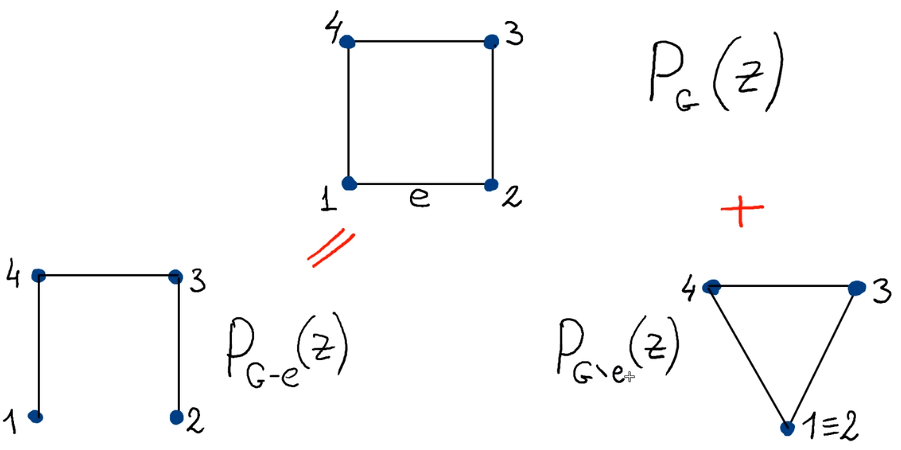
\includegraphics[width=10cm]{chromatic-polynome-rule.png}
		\caption{chromatic polynome rule}
	\end{figure}
	\hspace{1pt}
\end{proof}



\section{Планарные графы I}

\begin{definition}[Грань $f_i$] ...
\end{definition}

\begin{property}
	$ \sum{\deg(f_i)} = 2|E| \qquad ... = \sum{\deg(v_i)}$
\end{property}

\begin{theorem}
	Граница \iiany грани 2-связного плоского графа --- простой цикл
\end{theorem}

\begin{corollary}
	Вершины, смежные с \iiany вершиной 3-связного плоского графа -- лежат на простом цикле
\end{corollary}

\begin{definition}[Дуальный граф плоского графа]
	грани $\longrightarrow$ вершины; соединяем дуальные вершины ребром, если исходные грани смежны (т.е. отделены 1 ребром)
\end{definition}

\begin{property}
	Дуальный граф всегда связен; вершины $\longleftrightarrow$ грани (с сохранением степеней)
\end{property}

\begin{theorem}[Формула Эйлера для выпуклых многогранников и связных планарных графов]
	\[ V+F = E+2 \]
\end{theorem}

\begin{property}
	В простом плоском графе $\deg(f_i) \geqslant 3$
	\begin{itemize}
		\item $\deg(f_i)=1$ $\implies$ петля
		\item $\deg(f_i)=2$ $\implies$ мультиребро
	\end{itemize}
\end{property}

\begin{corollary}
	В простом плоском графе $E \leqslant 3V-6$; если равенство, то это \textbf{max} планарный граф
\end{corollary}

\begin{theorem}[Фэри / Fury]
	\iiany планарный граф можно так уложить в плоскость, что все рёбра -- прямые отрезки 
\end{theorem}

\begin{theorem}[о 4 красках]
	Для правильной раскраски граней плоского графа (без мостов) хватит 4 цветов
\end{theorem}

\begin{corollary}
	Плоский граф $\longrightarrow$ дуальный (грани $\Leftrightarrow$ вершины), а вершины плоского дуального графа $\Leftrightarrow$ вершинам его планарного. Так что задача $\equiv$ правильной раскраске \textbf{вершин} планарного графа
\end{corollary}



\section{Планарные графы II}

\iiTODO



\vspace{48pt} \noindent \hrulefill~ \raisebox{-8pt}[10pt][10pt]{\Huge\ding{102}}~ \hrulefill

\end{document}
